\documentclass[tikz]{standalone}
\usepackage{pgfplots}
\pgfplotsset{width=13cm,compat=1.18}
\begin{document}

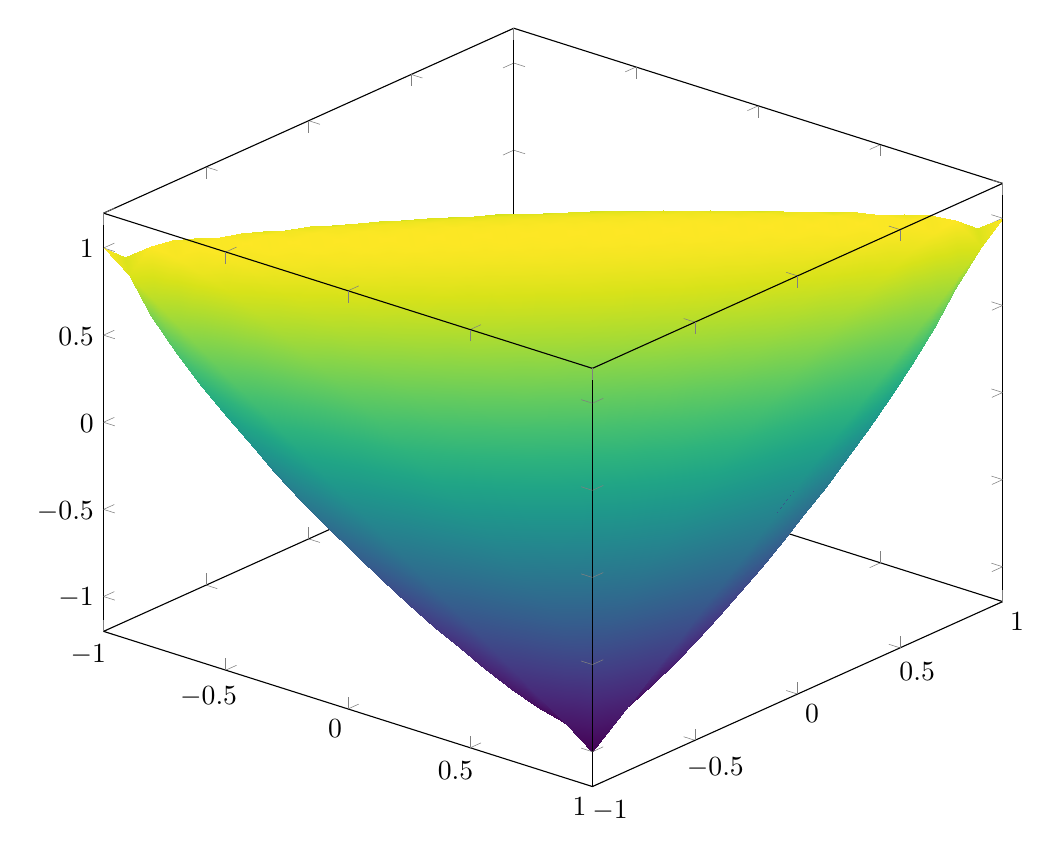
\begin{tikzpicture}
\begin{axis}
[ 
  % view={-45}{45},
  view/h=40,
  3d box=complete,
  % grid=major,
  colormap/viridis,
  samples=20,
  unit vector ratio=, %1 1 1,
  z post scale=1,
  z buffer=sort,
]

\addplot3 [surf,shader=interp,domain=-1:1] (
  {x},
  {y},
  {x*y - sqrt((x^2-1)*(y^2-1))}
);

\addplot3 [surf,shader=interp,domain=-1:1] (
  {x},
  {y},
  {x*y + sqrt((x^2-1)*(y^2-1))}
);

\end{axis}
\end{tikzpicture}

\end{document}
